\documentclass{article}

\usepackage{amsmath, amsthm, amssymb, amsfonts}
\usepackage{thmtools}
\usepackage{pgfplots}
\pgfplotsset{compat=1.17}
\usepackage{arabtex}
\usepackage{utf8}
\setcode{utf8}
\usepackage{tikz}
\usepackage{graphicx}
\usepackage{setspace}
\usepackage{geometry}
\usepackage{float}
\usepackage{hyperref}
\usepackage[utf8]{inputenc}
\usepackage[english]{babel}
\usepackage{framed}
\usepackage[dvipsnames]{xcolor}
\usepackage{tcolorbox}
\usepackage[table,xcdraw]{xcolor}
\tcbset{terminal/.style={
  colback=black, coltext=green, colframe=black,
  listing only, listing options={language=bash, basicstyle=\ttfamily}
}}
\usepackage{qrcode}      % For QR codes
\definecolor{spotifygreen}{RGB}{30,215,96} % Official Spotify Green
\usepackage{fontawesome5} % For Spotify icon and other FontAwesome 5 icons


\colorlet{LightGray}{White!90!Periwinkle}
\colorlet{LightOrange}{Orange!15}
\colorlet{LightGreen}{Green!15}

\newcommand{\HRule}[1]{\rule{\linewidth}{#1}}

\declaretheoremstyle[name=Theorem,]{thmsty}
\declaretheorem[style=thmsty,numberwithin=section]{theorem}
\tcolorboxenvironment{theorem}{colback=white}

\declaretheoremstyle[name=Corollary,]{thmsty}
\declaretheorem[style=thmsty,numberwithin=section]{corollary}
\tcolorboxenvironment{corollary}{colback=white}

\declaretheoremstyle[name=Theorem,]{thmsty}
\declaretheorem[style=thmsty,numberwithin=section]{subtheorem}
\tcolorboxenvironment{subtheorem}{colback=white}

\declaretheoremstyle[name=Proposition,]{prosty}
\declaretheorem[style=prosty,numberwithin=section]{proposition}
\tcolorboxenvironment{proposition}{colback=white}

\declaretheoremstyle[name=Principle,]{prcpsty}
\declaretheorem[style=prcpsty,numberlike=theorem]{principle}
\tcolorboxenvironment{principle}{colback=white}

\setstretch{1.2}
\geometry{
    textheight=9in,
    textwidth=5.5in,
    top=1in,
    headheight=12pt,
    headsep=25pt,
    footskip=30pt
}

% ------------------------------------------------------------------------------

\begin{document}

% ------------------------------------------------------------------------------
% Cover Page and ToC
% ------------------------------------------------------------------------------

\title{ \normalsize \textsc{}
		\\ [0cm]
		\HRule{1.5pt} \\
		\LARGE \noindent \textbf{\uppercase{Calculus \& analytical geometry (2)\\ (MATH 132)-Worksheet\#02}
		\HRule{2.0pt} \\ [0.6cm] \LARGE{Cairo University \\ Faculty Of Science} \vspace*{1\baselineskip}}
        \\
        
		}
        
\date{$3^{\text{rd}}$ week (February 22, 2025 - February 27, 2025)}

\author{ \noindent \textbf{Written \& Reviewed by} \\ 3ndlyb Alabyd} \\ 

\maketitle


\section*{Answer for Q1}

Evaluate the integral:
\[
\int_1^5 (4 - 2x) \, dx
\]
by interpreting it as a limit of a Riemann sum.

\subsection*{Step 1: Partition the Interval}
Divide the interval $[1, 5]$ into $n$ subintervals of equal width:
\[
\Delta x = \frac{5 - 1}{n} = \frac{4}{n}.
\]

The right endpoint of the $i$-th subinterval is:
\[
x_i = 1 + i \Delta x = 1 + \frac{4i}{n}.
\]

The Riemann sum is:
\[
S_n = \sum_{i=1}^n \left[4 - 2\left(1 + \frac{4i}{n}\right)\right] \Delta x.
\]

\subsection*{Step 2: Simplify the Summation}
Simplifying the integrand:
\[
4 - 2\left(1 + \frac{4i}{n}\right) = 2 - \frac{8i}{n}.
\]

The Riemann sum becomes:
\[
S_n = \sum_{i=1}^n \left(2 - \frac{8i}{n}\right) \cdot \frac{4}{n}.
\]

Distribute $\frac{4}{n}$:
\[
S_n = \sum_{i=1}^n \left(\frac{8}{n} - \frac{32i}{n^2}\right).
\]

Separate the sums:
\[
S_n = \frac{8}{n} \sum_{i=1}^n 1 - \frac{32}{n^2} \sum_{i=1}^n i.
\]

Using known summations:
\[
\sum_{i=1}^n 1 = n \quad \text{and} \quad \sum_{i=1}^n i = \frac{n(n+1)}{2},
\]
we get:
\[
S_n = \frac{8}{n} \cdot n - \frac{32}{n^2} \cdot \frac{n(n+1)}{2}.
\]

Simplify:
\[
S_n = 8 - \frac{32(n+1)}{2n} = 8 - \frac{16(n+1)}{n}.
\]

\subsection*{Step 3: Taking the Limit}
Taking the limit as $n \to \infty$:
\[
\lim_{n \to \infty} S_n = \lim_{n \to \infty} \left[8 - \frac{16(n+1)}{n}\right].
\]

Simplify the expression:
\[
= \lim_{n \to \infty} \left[8 - 16\left(1 + \frac{1}{n}\right)\right]
= 8 - 16 = -8.
\]


\subsection*{Final Answer}
\[
\boxed{-8}
\]
\section*{Answer for Q2}
Evaluate the integral:
\[
\int_1^5 (x^2 - 4x + 2) \, dx
\]

\subsection*{Step 1: Partition the Interval}
Divide the interval $[1,5]$ into $n$ equal subintervals:
\[
\Delta x = \frac{5 - 1}{n} = \frac{4}{n}.
\]
The right endpoint of the $k$-th subinterval is:
\[
x_k = 1 + \frac{4k}{n}, \quad k = 0,1,2,\dots,n.
\]

\subsection*{Step 2: Riemann Sum Representation}
The Riemann sum using right endpoints is:
\[
S_n = \sum_{k=1}^{n} \left[ \left(1 + \frac{4k}{n}\right)^2 - 4\left(1 + \frac{4k}{n}\right) + 2 \right] \cdot \frac{4}{n}.
\]

\subsection*{Step 3: Expand the Function}
Expand and simplify:
\[
\left(1 + \frac{4k}{n}\right)^2 = 1 + \frac{8k}{n} + \frac{16k^2}{n^2}.
\]
Thus:
\[
x_k^2 - 4x_k + 2 = 1 + \frac{8k}{n} + \frac{16k^2}{n^2} - 4 - \frac{16k}{n} + 2.
\]
\[
= \frac{16k^2}{n^2} - \frac{8k}{n} - 1.
\]

\subsection*{Step 4: Full Riemann Sum}
\[
S_n = \sum_{k=1}^{n} \left( \frac{16k^2}{n^2} - \frac{8k}{n} - 1 \right) \cdot \frac{4}{n}.
\]
\[
= \sum_{k=1}^{n} \left( \frac{64k^2}{n^3} - \frac{32k}{n^2} - \frac{4}{n} \right).
\]

\subsection*{Step 5: Apply Summation Formulas}
Use:
\[
\sum_{k=1}^{n} k = \frac{n(n+1)}{2}, \quad \sum_{k=1}^{n} k^2 = \frac{n(n+1)(2n+1)}{6}.
\]

Substituting:
\[
S_n = \frac{64}{n^3} \cdot \frac{n(n+1)(2n+1)}{6} - \frac{32}{n^2} \cdot \frac{n(n+1)}{2} - \frac{4}{n} \cdot n.
\]

Simplifying:
\[
S_n = \frac{64(n+1)(2n+1)}{6n^2} - \frac{16(n+1)}{n} - 4.
\]

\subsection*{Step 6: Taking the Limit}
As $n \to \infty$:
\[
\lim_{n \to \infty} S_n = \frac{64 \cdot 2}{6} - 16 - 4 = \frac{128}{6} - 20 = \frac{64}{3} - 20 = \frac{4}{3}.
\]

\subsection*{Final Answer}
\[
\boxed{\frac{4}{3}}
\]
\section*{Answer of Q3}

\subsection*{Step 1: Set up the Riemann sum}

Consider the interval $[a,b]$ divided into $n$ equal subintervals. \\ The width of each subinterval is:
\[
\Delta x = \frac{b - a}{n}.
\]

The right endpoint of the $i$-th subinterval is:
\[
x_i = a + i \Delta x=a + i\frac{b - a}{n}.
\]

\subsection*{Step 2: Write the Riemann sum}

The Riemann sum using right endpoints is:
\[
S_n = \sum_{i=1}^{n} (x_i)^2 \Delta x.
\]

Substituting $x_i$:
\[
S_n = \sum_{i=1}^{n} \left(a + i\frac{b-a}{n}\right)^2 \cdot \frac{b-a}{n}.
\]

\subsection*{Step 3: Expand and simplify}

Expand the square:
\[
\left(a + i\frac{b-a}{n}\right)^2 = a^2 + 2a\frac{b-a}{n}i + \left(\frac{b-a}{n}\right)^2 i^2.
\]

Thus:
\[
S_n = \frac{b-a}{n} \sum_{i=1}^{n} \left[ a^2 + 2a\frac{b-a}{n}i + \left(\frac{b-a}{n}\right)^2 i^2 \right].
\]

\subsection*{Step 4: Use known summation formulas}

Using the standard summation formulas:
\[
\sum_{i=1}^{n} 1 = n, \quad \sum_{i=1}^{n} i = \frac{n(n+1)}{2}, \quad \sum_{i=1}^{n} i^2 = \frac{n(n+1)(2n+1)}{6},
\]

we get:
\[
S_n = \frac{b-a}{n} \left[ a^2 n + 2a\frac{b-a}{n}\cdot \frac{n(n+1)}{2} + \left(\frac{b-a}{n}\right)^2 \cdot \frac{n(n+1)(2n+1)}{6} \right].
\]

\subsection*{Step 5: Simplify the expression}

Simplifying:
\[
S_n = (b-a)\left[ a^2 + a(b-a)\frac{n+1}{n} + \frac{(b-a)^2}{n^2}\frac{(n+1)(2n+1)}{6} \right].
\]

\subsection*{Step 6: Take the limit as $n \to \infty$}
As $n \to \infty$:
\[
\frac{n+1}{n} \to 1, \quad \text{and} \quad \frac{(n+1)(2n+1)}{n^2} \to 2.
\]

Hence:
\[
\lim_{n \to \infty} S_n = (b-a)\left[ a^2 + a(b-a) + \frac{(b-a)^2}{3} \right].
\]

Expanding:
\[
= (b-a)\left( a^2 + ab - a^2 + \frac{b^2 - 2ab + a^2}{3} \right),
\]
\[
= (b-a)\frac{b^2 + ab + a^2}{3}.
\]

\subsection*{Step 7: Recognize the factorization}

Since:
\[
b^3 - a^3 = (b-a)(b^2 + ab + a^2),
\]

we have:
\[
\lim_{n \to \infty} S_n = \frac{b^3 - a^3}{3}.
\]
\subsection*{Final Answer:}
\[
\boxed{\int_a^b x^2 \, dx = \frac{b^3 - a^3}{3}}.
\]

    

\section*{Answer of Q4}

\subsection*{Step 1: Partition the Interval}
We partition the interval \([1, 2]\) into \(n\) subintervals of equal length. The width of each subinterval is:
\[
\Delta x = \frac{2 - 1}{n} = \frac{1}{n}.
\]

\subsection*{Step 2: Choose Sample Points}
Let \(x_i\) be the right endpoint of the \(i\)-th subinterval:
\[
x_i = 1 + i \Delta x = 1 + \frac{i}{n}, \quad i = 1, 2, \ldots, n.
\]

\subsection*{Step 3: Write the Riemann Sum}
The Riemann sum for the given integral is:
\[
\sum_{i=1}^{n} \sqrt{4 - \left(1 + \frac{i}{n}\right)^2} \cdot \frac{1}{n}.
\]

\subsection*{Step 4: Take the Limit of the Riemann Sum}
Taking the limit as \(n \to \infty\), we get:
\[
\int_1^2 \sqrt{4 - x^2} \, dx 
= \lim_{n \to \infty} \sum_{i=1}^{n} \sqrt{4 - \left(1 + \frac{i}{n}\right)^2} \cdot \frac{1}{n}.
\]

\subsection*{Final Answer}
\[
\boxed{\int_1^2 \sqrt{4 - x^2} \, dx 
= \lim_{n \to \infty} \sum_{i=1}^{n} \sqrt{4 - \left(1 + \frac{i}{n}\right)^2} \cdot \frac{1}{n}.}
\]
\section*{Answer of Q5}

\subsection*{Step 1: Divide the Interval}
Divide the interval \([2,5]\) into \(n\) subintervals of equal width:
\[
\Delta x = \frac{5 - 2}{n} = \frac{3}{n}.
\]

\subsection*{Step 2: Choose Sample Points}
Choose the right-endpoint for each subinterval as the sample point:
\[
x_i^* = 2 + i \Delta x = 2 + \frac{3i}{n}, \quad \text{for } i = 1, 2, \dots, n.
\]

\subsection*{Step 3: Write the Riemann Sum}
The Riemann sum corresponding to the given function \(f(x) = x^2 + \frac{1}{x}\) is:
\[
\sum_{i=1}^n \left[ \left(x_i^*\right)^2 + \frac{1}{x_i^*} \right] \Delta x.
\]

Substituting \(x_i^*\) and \(\Delta x\):
\[
\sum_{i=1}^n \left[ \left(2 + \frac{3i}{n}\right)^2 + \frac{1}{2 + \frac{3i}{n}} \right] \cdot \frac{3}{n}.
\]

\subsection*{Step 4: Express as a Limit}
Finally, expressing the integral as a limit of Riemann sums:
\[
\int_2^5 \left( x^2 + \frac{1}{x} \right) \, dx = \lim_{n \to \infty} \sum_{i=1}^n \left[ \left(2 + \frac{3i}{n}\right)^2 + \frac{1}{2 + \frac{3i}{n}} \right] \frac{3}{n}.
\]

\subsection*{Final Answer}
\[
\boxed{
\int_2^5 \left( x^2 + \frac{1}{x} \right) \, dx = \lim_{n \to \infty} \sum_{i=1}^n \left[ \left(2 + \frac{3i}{n}\right)^2 + \frac{1}{2 + \frac{3i}{n}} \right] \frac{3}{n}.}
\]
\section*{Answer for Q6}
\subsection*{(a)}
\subsubsection*{Step 1: Identify the Riemann Sum Structure}
A Riemann sum typically has the form:
\[
\sum_{k=1}^n f(x_k) \Delta x,
\]
where:
\begin{itemize}
    \item \(\Delta x = \frac{b - a}{n}\),
    \item \(x_k = a + k \Delta x\),
    \item The limit as \(n \to \infty\) gives the integral \(\int_a^b f(x) \, dx\).
\end{itemize}

In our case:
\begin{itemize}
    \item \(\Delta x = \frac{1}{n}\),
    \item Let \(x_k = \frac{k}{n}\), so that as \(n \to \infty\), \(x_k\) ranges from 0 to 1,
    \item The expression inside the sum becomes \(3x_k + 2\).
\end{itemize}

\subsubsection*{Step 2: Write the Limit as a Riemann Sum}
Thus, the sum can be rewritten as:
\[
\frac{1}{n}\sum_{k=1}^n \left(3 \cdot \frac{k}{n} + 2\right) 
= \sum_{k=1}^n \left(3x_k + 2\right) \frac{1}{n}.
\]

This is precisely the Riemann sum for the integral:
\[
\int_0^1 (3x + 2) \, dx.
\]

\subsubsection*{Final Answer}

\[
\boxed{\int_0^1 (3x + 2) \, dx.}
\]
\subsection*{(b)}
\subsubsection*{Step 1: Recognizing the Riemann Sum Form}

The given limit can be rewritten as:

\begin{equation*}
\lim_{n \to \infty}\sum_{k=1}^n \frac{1}{1+\left( \frac{k}{n} \right)^2} \cdot \frac{1}{n}.
\end{equation*}

This resembles a Riemann sum of the form:

\[
\sum_{k=1}^n f(x_k) \Delta x,
\]

where:
\[
x_k = \frac{k}{n} \quad \text{and} \quad \Delta x = \frac{1}{n}.
\]

\subsubsection*{Step 2: Converting to the Integral}

As \(n \to \infty\), the Riemann sum approaches the definite integral:

\begin{equation*}
\int_0^1 \frac{1}{1 + x^2} \, dx.
\end{equation*}

\subsubsection*{Final Answer}

Thus, the given limit can be expressed as the integral:

\begin{equation*}
\boxed{\int_0^1 \frac{1}{1 + x^2} \, dx.}
\end{equation*}
\section*{Answer for Q7}
\begin{itemize}
    \item a) \quad 4\\
    \item b) \quad 10\\
    \item c) \quad -3\\
    \item d) \quad 3
\end{itemize}
It is left to the reader to verify this by counting the squares. You can find the area bounded by an inclined line by simply counting the squares in the surrounding rectangle and dividing by 2. Refer to the figure for further clarification\\
\begin{center}
    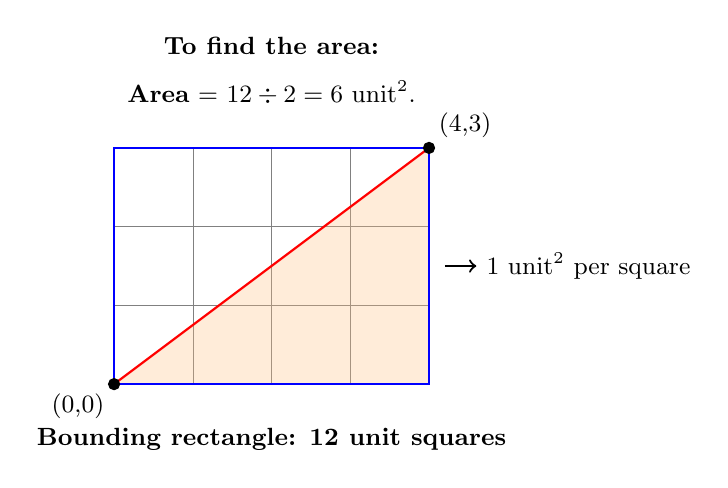
\begin{tikzpicture}
    % Draw the grid
    \draw[step=1cm,gray,very thin] (0,0) grid (4,3);


    % Shade the triangle area
    \fill[orange!50, opacity = 0.3] (0,0) -- (4,3) -- (4,0) -- cycle;


    % Draw the bounding rectangle
    \draw[thick, blue] (0,0) rectangle (4,3);
    \node at (2,-0.7) {\small \textbf{Bounding rectangle: 12 unit squares}};

    % Draw the inclined line (hypotenuse)
    \draw[thick, red] (0,0) -- (4,3);

    % Mark key points
    \filldraw[black] (0,0) circle (2pt) node[below left]{\small (0,0)};
    \filldraw[black] (4,3) circle (2pt) node[above right]{\small (4,3)};

    % Add explanation above the figure
    \node at (2,4.3) {\small \textbf{To find the area:}};

    \node at (2,3.7) {\small \textbf{Area} = $12 \div 2 = 6$ unit$^2$.};

    % Arrows to highlight counting squares
    \draw[->, thick] (4.2,1.5) -- (4.6,1.5) node[right]{\small 1 unit$^2$ per square};

\end{tikzpicture}
\end{center}
\section*{Answer for Q8}
\subsection*{Step 1: Geometric Interpretation}
The integrand \(\sqrt{9 - x^2}\) represents the upper half of a circle centered at the origin with radius \(r = 3\). The full equation of the circle is:
\[
x^2 + y^2 = 9.
\]

Since the integral bounds are from \(-3\) to \(3\), the integral represents the area under the upper semicircle of this circle.
\begin{center}
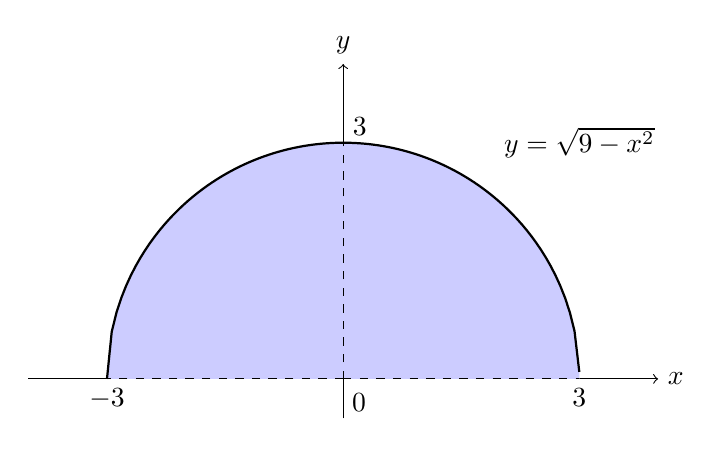
\begin{tikzpicture}[scale=1]
    % Axes
    \draw[->] (-4,0) -- (4,0) node[right] {$x$};
    \draw[->] (0,-0.5) -- (0,4) node[above] {$y$};



    % Shaded area under the curve
    \begin{scope}
        \clip (-3,0) rectangle (3,3);
        \fill[blue!20, domain=-3:3, samples=100] 
            plot (\x, {sqrt(9 - \x*\x)}) -- (3,0) -- (-3,0) -- cycle;
    \end{scope}
    % Upper semicircle
    \draw[thick, domain=-3:3, samples=100] 
        plot (\x, {sqrt(9 - \x*\x)});
    \node at (3,3)  {$y=\sqrt{9-x^2}$};
    % Radius indicators
    \draw[dashed] (0,0) -- (3,0) node[left, below] {$3$};
    \draw[dashed] (0,0) -- (-3,0) node[left, below] {$-3$};
    \draw[dashed] (0,0) -- (0,3.2) node[above, right] {$3$};

    % Labels
    \node at (0.2,-0.3) {0};
\end{tikzpicture}
\end{center}
\subsection*{Step 2: Area of the Corresponding Circle}
The area of a full circle with radius \(r\) is given by:
\[
\text{Area of a full circle} = \pi r^2.
\]

Substituting \(r = 3\):
\[
\text{Area} = \pi \times 3^2 = 9\pi.
\]

\subsection*{Step 3: Area of the Upper Semicircle}
Since the integral corresponds to the area of the upper half of the circle, we take half of the total area:
\[
\text{Area of upper semicircle} = \frac{1}{2} \times 9\pi = \frac{9\pi}{2}.
\]

\subsection*{Final Answer}
Thus, the value of the integral is:
\[
\boxed{\frac{9\pi}{2}}.
\]
\section*{Answer of Q9}
\subsection*{Step 1: Analyze the Graph of \(y = 4 - |x|\)}
The function \(y = 4 - |x|\) forms a ``V"-shaped graph symmetric about the \(y\)-axis. Key points on the graph are:
\begin{itemize}
    \item At \(x = 0\), \(y = 4\).
    \item At \(x = \pm 2\), \(y = 2\).
\end{itemize}
The graph decreases linearly from \(y = 4\) at \(x = 0\) to \(y = 2\) at \(x = \pm 2\).



\subsection*{Step 2: Geometric Decomposition}
We can interpret the region under the graph as the combination of:
\begin{enumerate}
    \item A \textbf{rectangle} with:
    \begin{itemize}
        \item Width = 4 (from \(-2\) to \(2\)).
        \item Height = 2 (since \(y = 2\) at the endpoints).
    \end{itemize}
    Therefore, the area of the rectangle is:
    \[
    A_{\text{rectangle}} = \text{width} \times \text{height} = 4 \times 2 = 8.
    \]

    \item A \textbf{triangle} above the rectangle with:
    \begin{itemize}
        \item Base = 4 (from \(-2\) to \(2\)).
        \item Height = 2 (from \(y = 2\) to \(y = 4\)).
    \end{itemize}
    The area of the triangle is:
    \[
    A_{\text{triangle}} = \frac{1}{2} \times \text{base} \times \text{height}
    = \frac{1}{2} \times 4 \times 2 = 4.
    \]
\end{enumerate}
\begin{center}
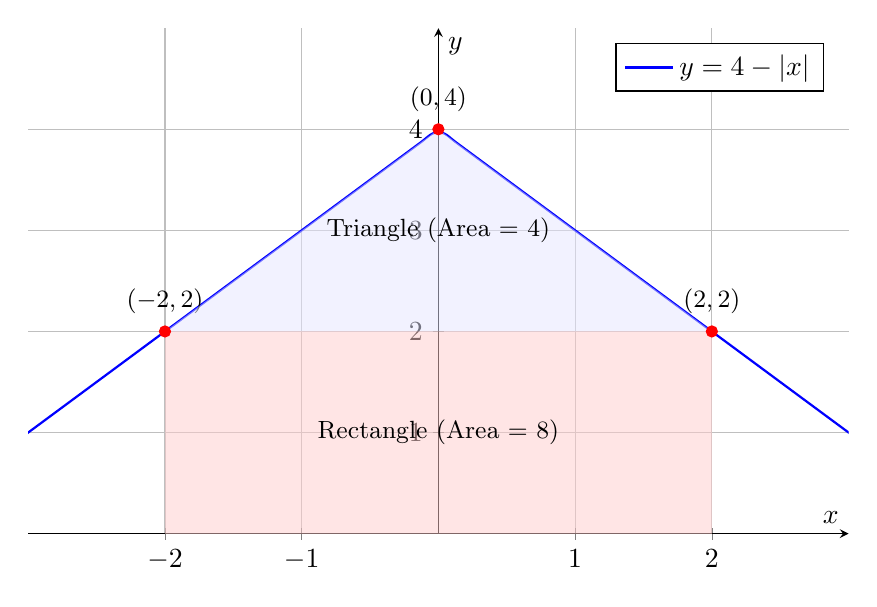
\begin{tikzpicture}
    \begin{axis}[
        axis lines = middle,
        xlabel = {$x$},
        ylabel = {$y$},
        ymin = 0, ymax = 5,
        xmin = -3, xmax = 3,
        xtick = {-2,-1,0,1,2},
        ytick = {0,1,2,3,4},
        domain = -4:4,
        samples = 100,
        width=12cm,
        height=8cm,
        grid = major,
        legend pos = north east
    ]
    % Plot of the function y = 4 - |x|
    \addplot[blue, thick, smooth] {4 - abs(x)};
    \addlegendentry{$y = 4 - |x|$}

    % Key points
    \addplot[
        only marks,
        mark=*,
        mark size=2pt,
        color=red
    ] coordinates {(-2,2) (0,4) (2,2)};

    % Annotations for key points
    \node at (axis cs:0,4.3) {\small $(0,4)$};
    \node at (axis cs:-2,2.3) {\small $(-2,2)$};
    \node at (axis cs:2,2.3) {\small $(2,2)$};

    % Rectangle shading
    \addplot [
        ybar,
        bar width=4,
        fill=red!20,
        opacity=0.5,
        draw=none
    ] coordinates {(0,2)};

    % Triangle shading
    \path [fill=blue!10, opacity=0.5] 
        (axis cs:-2,2) -- (axis cs:0,4) -- (axis cs:2,2) -- cycle;

    % Labels for shapes
    \node at (axis cs:0,1) {\small Rectangle (Area = 8)};
    \node at (axis cs:0,3) {\small Triangle (Area = 4)};
    \end{axis}
\end{tikzpicture}
\end{center}

\subsection*{Step 3: Total Area}
The total area under the curve (and hence the value of the integral) is the sum of the rectangle's area and the triangle's area:
\[
A_{\text{total}} = A_{\text{rectangle}} + A_{\text{triangle}} = 8 + 4 = 12.
\]


\subsection*{Final Answer}
Thus, the value of the integral is:
\[
\int_{-2}^2 (4 - |x|) \, dx = \boxed{12}.
\]
\section*{Answer of Q10}
We are given the following integrals:
\[
\int_2^8 f(x)\,dx = 7.3 \quad \text{and} \quad \int_2^4 f(x)\,dx = 5.9
\]

Using the property of definite integrals:
\[
\int_a^b f(x)\,dx = \int_a^c f(x)\,dx + \int_c^b f(x)\,dx
\]

Let $a = 2$, $b = 8$, and $c = 4$. Then:
\[
\int_2^8 f(x)\,dx = \int_2^4 f(x)\,dx + \int_4^8 f(x)\,dx
\]

Substitute the given values:
\[
7.3 = 5.9 + \int_4^8 f(x)\,dx
\]

Solving for $\int_4^8 f(x)\,dx$:
\[
\int_4^8 f(x)\,dx = 7.3 - 5.9 = 1.4
\]

\noindent\textbf{Final Answer:}
\[
\boxed{1.4}
\]
\section*{Anser for Q11}
\subsection*{Step 1: Split the integral}
\[
\int_{-3}^3 \left(4f(x) - 2g(x) + 5x^3\right) \, dx 
= 4\int_{-3}^3 f(x) \, dx - 2\int_{-3}^3 g(x) \, dx + \int_{-3}^3 5x^3 \, dx
\]

\subsection*{Step 2: Compute \(\int_{-3}^3 f(x) \, dx\)}
Given:
\[
\int_{-3}^2 f(x) \, dx = 10 \quad \text{and} \quad \int_2^3 f(x) \, dx = -4
\]

Thus:
\[
\int_{-3}^3 f(x) \, dx = \int_{-3}^2 f(x) \, dx + \int_2^3 f(x) \, dx = 10 + (-4) = 6
\]

\subsection*{Step 3: Compute \(\int_{-3}^3 g(x) \, dx\)}
Given:
\[
\int_3^{-3} g(x) \, dx = -2
\]

Reversing the limits:
\[
\int_{-3}^3 g(x) \, dx = -\int_3^{-3} g(x) \, dx = -(-2) = 2
\]

\subsection*{Step 4: Compute \(\int_{-3}^3 5x^3 \, dx\)}
Since \(x^3\) is an odd function, \(5x^3\) is also odd. The integral of an odd function over a symmetric interval \([-a, a]\) is 0:
\[
\int_{-3}^3 5x^3 \, dx = 0
\]

\subsection*{Step 5: Combine all results}
\[
\int_{-3}^3 \left(4f(x) - 2g(x) + 5x^3\right) \, dx 
= 4 \cdot 6 - 2 \cdot 2 + 0
= 24 - 4
= 20
\]

\subsection*{Final Answer}
\[
\boxed{20}
\]
\section*{Answer for Q12}
\subsection*{Defining the Functions}

Let the functions \( f \) and \( g \) on the interval \([0,1]\) be defined as follows:
\[
f(x) = \begin{cases} 
1 & \text{if } x \in \mathbb{Q}, \\[6pt]
0 & \text{if } x \in \mathbb{R} \setminus \mathbb{Q}\footnotemark,
\end{cases}
\]
\footnotetext{The notation \(\setminus\) denotes the set difference. Specifically, \(\mathbb{R} \setminus \mathbb{Q}\) represents the set of real numbers excluding the rational numbers, i.e., the set of irrational numbers.}
\[
g(x) = \begin{cases} 
-1 & \text{if } x \in \mathbb{Q}, \\[6pt]
0 & \text{if } x \in \mathbb{R} \setminus \mathbb{Q}.
\end{cases}
\]

\subsection*{Why \( f \) and \( g \) are Not Integrable on \([0,1]\)?}

\begin{itemize}
    \item Both \( f \) and \( g \) are examples of Dirichlet-type functions.
    \item For any partition of \([0,1]\), the upper and lower Riemann sums for \( f \) and \( g \) differ, implying that neither \( f \) nor \( g \) is Riemann integrable on \([0,1]\).
    \item More precise explanation that the set of rational numbers (\(\mathbb{Q}\)) is dense in \([0,1]\) and has measure zero.
\end{itemize}

\subsection*{Consider the Sum \( f + g \)}

Now, consider:
\[
(f + g)(x) = f(x) + g(x) = \begin{cases}
1 + (-1) = 0 & \text{if } x \in \mathbb{Q}, \\[6pt]
0 + 0 = 0 & \text{if } x \in \mathbb{R} \setminus \mathbb{Q}.
\end{cases}
\]

Hence, the sum simplifies to:
\[
(f + g)(x) = 0 \quad \text{for all } x \in [0,1].
\]


\noindent
Since \( (f + g)(x) = 0 \) for all \( x \) in \([0,1]\), it is the zero function, which is continuous and hence Riemann integrable. 
\section*{Answer for Q13}

Consider the function:
\[
f(x) = \begin{cases}
1 & \text{if } x \in \mathbb Q, \\[6pt]
-1 & \text{if } x \in \mathbb R \setminus \mathbb Q .
\end{cases}
\]

\subsection*{Why $f(x)$ is not Riemann integrable:}
\begin{itemize}
    \item Both rational and irrational numbers are dense in $[0,1]$.
    \item In every subinterval, $f(x)$ takes values $1$ (rationals) and $-1$ (irrationals).
    \item The function keeps oscillating between $1$ and $-1$ without settling, so the Riemann integral does not exist.
\end{itemize}

\subsection*{Why $|f(x)|$ is Riemann integrable:}
The absolute value is:
\[
|f(x)| = \begin{cases}
1 & \text{if } x \in \mathbb Q, \\[6pt]
1 & \text{if } x \in \mathbb R \setminus \mathbb Q .
\end{cases}
\]

This simplifies to:
\[
|f(x)| = 1 \quad \text{for all } x \in [0,1].
\]

Since $|f(x)|$ is the constant function $1$, it is Riemann integrable.
\section*{Answer for Q14}

\subsection*{Step 1: Prove the inequality \(1 \leq \sqrt{1+x^2} \leq \sqrt{2}\)}
Given:
\[
-1 \leq x \leq 1
\]

Squaring all sides gives:
\[
0 \leq x^2 \leq 1
\]

Adding 1 to all sides:
\[
1 \leq 1 + x^2 \leq 2
\]

Taking the square root of all sides (since all terms are non-negative, we keep the positive root):
\[
1 \leq \sqrt{1+x^2} \leq \sqrt{2}
\]

\subsection*{Step 2: Use properties of integrals to establish the given inequality}

Since for all \(x\) in \([-1, 1]\):
\[
1 \leq \sqrt{1+x^2} \leq \sqrt{2},
\]

we can use the \textbf{comparison property of integrals}, which states:

\medskip
\noindent
\textit{If \(f(x)\) is continuous on \([a,b]\) and \(m \leq f(x) \leq M\) for all \(x \in [a,b]\), then:}
\[
m(b - a) \leq \int_a^b f(x) \, dx \leq M(b - a)
\]

\medskip
\noindent
In our case:
\[
f(x) = \sqrt{1+x^2}, \quad m = 1, \quad M = \sqrt{2}, \quad a = -1, \quad b = 1.
\]

The length of the interval is:
\[
b - a = 1 - (-1) = 2.
\]

Thus:
\[
1 \times 2 \leq \int_{-1}^1 \sqrt{1+x^2} \, dx \leq \sqrt{2} \times 2
\]

\[
2 \leq \int_{-1}^1 \sqrt{1+x^2} \, dx \leq 2\sqrt{2}
\]

\subsection*{Final Answer}
\[
\boxed{2 \leq \int_{-1}^1 \sqrt{1+x^2} \, dx \leq 2\sqrt{2}}
\]
\section*{Answer for Q15}
\begin{proposition}
If $f$ is continuous on $[a,b]$, then
\[
\left| \int_a^b f(x) \, dx \right| \leq \int_a^b |f(x)| \, dx.
\]
\end{proposition}


\begin{proof}
    \begin{enumerate}
    \item \textbf{Start with the given inequality:} \\
    From the given hint, we have:
    \[
    -|f(x)| \leq f(x) \leq |f(x)|.
    \]

    \item \textbf{Integrate over $[a,b]$:} \\
    Since the integral preserves inequalities, we obtain:
    \[
    \int_a^b -|f(x)| \, dx \leq \int_a^b f(x) \, dx \leq \int_a^b |f(x)| \, dx.
    \]

    \item \textbf{Simplify the inequality:} \\
    The integral of $-|f(x)|$ is simply the negative of the integral of $|f(x)|$:
    \[
    -\int_a^b |f(x)| \, dx \leq \int_a^b f(x) \, dx \leq \int_a^b |f(x)| \, dx.
    \]

    \item \textbf{Apply the equivalence $-b \leq a \leq b \iff |a| \leq b$:} \\
    Since we have:
    \[
    -\int_a^b |f(x)| \, dx \leq \int_a^b f(x) \, dx \leq \int_a^b |f(x)| \, dx,
    \]
    it follows by the equivalence $-b \leq a \leq b \iff |a| \leq b$ that:
    \[
    \left| \int_a^b f(x) \, dx \right| \leq \int_a^b |f(x)| \, dx.
    \]
\end{enumerate}
\end{proof}
\begin{theorem}\label{thm:main_theorem}
    If $f$ is continuous on $[a,b]$, then
\[
\left| \int_a^b f(x) \, dx \right| \leq \int_a^b |f(x)| \, dx.
\]
\end{theorem}

We want to show that
\[
\left| \int_0^{2\pi} f(x)\sin(2x) \, dx \right| \leq \int_0^{2\pi} |f(x)| \, dx.
\]
\proof
\subsection*{Step 1: Define a Suitable Function}
Let 
\[
g(x) = f(x)\sin(2x).
\]
Since $f(x)$ is continuous on $[0, 2\pi]$ and $\sin(2x)$ is also continuous on $[0, 2\pi]$, their product $g(x)$ is continuous on $[0, 2\pi]$.

\subsection*{Step 2: Apply \texorpdfstring{\hyperref[thm:main_theorem]{Theorem~\ref*{thm:main_theorem}}}{Theorem}}
By applying \hyperref[thm:main_theorem]{Theorem~\ref*{thm:main_theorem}} to $g(x)$, we have:
\[
\left| \int_0^{2\pi} g(x) \, dx \right| \leq \int_0^{2\pi} |g(x)| \, dx.
\]

Substituting $g(x) = f(x)\sin(2x)$:
\[
\left| \int_0^{2\pi} f(x)\sin(2x) \, dx \right| \leq \int_0^{2\pi} |f(x)\sin(2x)| \, dx.
\]

\subsection*{Step 3: Simplify the Absolute Value}
Since $|\sin(2x)| \leq 1$ for all $x$, we have:
\[
|f(x)\sin(2x)| = |f(x)| \cdot |\sin(2x)| \leq |f(x)|.
\]

Thus:
\[
\int_0^{2\pi} |f(x)\sin(2x)| \, dx \leq \int_0^{2\pi} |f(x)| \, dx.
\]

\subsection*{Step 4: Combine the Inequalities}
Combining the inequalities from the previous steps:
\[
\left| \int_0^{2\pi} f(x)\sin(2x) \, dx \right| \leq \int_0^{2\pi} |f(x)| \, dx.
\]

\subsection*{Final Answer}
Hence, we have shown that:
\[
\boxed{\left| \int_0^{2\pi} f(x)\sin(2x) \, dx \right| \leq \int_0^{2\pi} |f(x)| \, dx.}
\]

\qed
\section*{About The Repository}

This document is part of the \href{https://github.com/3ndlyb/Math132Answers}{\texttt{github.com/3ndlyb/Math132Answers}} repository, which contains solutions to Math132 problem sheets. Each sheet is organized in its own folder, including:

\begin{itemize}
    \item The original problem sheet in PDF format (\texttt{Math - 132 - sheetX.pdf}).
    \item A \LaTeX{} source file (\texttt{main.tex}) containing the answers.
    \item The compiled PDF of the answers (\texttt{SheetXAns.pdf}).
\end{itemize}

To view the answers, simply open the corresponding \texttt{SheetXAns.pdf} file. If you wish to edit the answers, you can modify the \texttt{main.tex} file and recompile it using:

\begin{tcolorbox}[terminal]
\begin{verbatim}
$ pdflatex main.tex
\end{verbatim}
\end{tcolorbox}


Make sure you have a suitable \LaTeX{} distribution installed, such as TeX Live or MiKTeX.

\subsection*{Contributions and Feedback}

Contributions to improve the repository are welcome. If you spot any errors or have suggestions, feel free to:
\begin{enumerate}
    \item Open an issue on the GitHub repository.
    \item Fork the repository, make your changes, and submit a pull request.
\end{enumerate}

The repository is licensed under the MIT License, so you are free to use, modify, and share the materials.  

\subsection*{Contact}

For further questions or feedback, feel free to reach out via Discord at \boxed{\texttt{3ndlybalabyd}} \! .
\definecolor{spotifygreen}{RGB}{30,215,96} % Official Spotify Green

\section*{Acknowledgments}

\begin{tcolorbox}[
    colback=black,         % Background color
    colframe=spotifygreen, % Border color (Spotify green)
    width=\textwidth,      % Full width
    boxrule=1mm,           % Border thickness
    sharp corners=south,   % Rounded top corners only
    arc=5mm,               % Curve radius for corners
    fontupper=\color{white}\sffamily, % White sans-serif text
    title=\textbf{\huge \textcolor{white}{\faSpotify} \begin{arabtext}
anaa kryb anaa wyrdw
\end{arabtext}},
    coltitle=white,        % Title text color
    attach boxed title to top left={yshift=-2mm, xshift=5mm},
    boxed title style={colback=black, sharp corners}
]
    \begin{center}
        % ------ PLAYLIST COVER IMAGE ------
        
\includegraphics[width=4cm,clip,trim=0 0 0 0]{playlist_cover.jpeg}

        \vspace{0.5cm}

        % ------ DESCRIPTION ------
        This document wouldn't have been possible without this beloved Spotify playlist of just Radiohead songs.\\ Click the link below or scan the QR code to listen to it:

        \vspace{0.5cm}

        % ------ CLICKABLE LINK ------
        \href{https://open.spotify.com/playlist/7CmaLgwblAvazjCSSjy3Ja}{%
            \textcolor{spotifygreen}{\Large \textbf{Listen on Spotify}}%
        }

        \vspace{0.5cm}

        % ------ QR CODE ------
        \qrcode[height=3cm]{https://open.spotify.com/playlist/7CmaLgwblAvazjCSSjy3Ja}
    \end{center}
\end{tcolorbox}

\end{document}
